\chapter{Polut ja kierrokset}

Verkkoteorian syntyhetkenä pidetään vuotta 1736,
jolloin matemaatikko
Leonhard Euler tutki Königsbergin siltaongelmaa.
Tehtävänä oli etsiä reitti,
joka kulkisi tarkalleen kerran
kaupungin seitsemän sillan yli.
Euler esitti tilanteen verkkona ja
osoitti, ettei halutunlaista reittiä ole olemassa.

Eulerin analyysi tarjoaa yleisen menetelmän tutkia,
onko verkossa polkua, joka kulkee tarkalleen kerran
jokaista kaarta pitkin.
Osoittautuu, että polun olemassaolon voi päätellä
suoraan verkon solmujen asteista,
ja jos polku on olemassa, sen pystyy myös
muodostamaan tehokkaasti.

\section{Käsitteitä}

\index{Eulerin polku}

Eulerin polku (\textit{Eulerian path}) on verkossa oleva
polku, joka kulkee tarkalleen kerran jokaista kaarta pitkin.
Esimerkiksi verkossa
\begin{center}
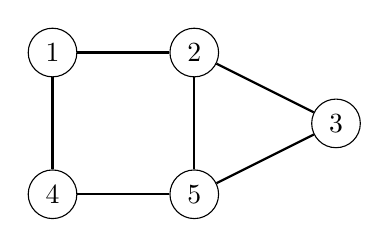
\begin{tikzpicture}[scale=0.9]
\node[draw, circle] (1) at (1,5) {$1$};
\node[draw, circle] (2) at (3,5) {$2$};
\node[draw, circle] (3) at (5,4) {$3$};
\node[draw, circle] (4) at (1,3) {$4$};
\node[draw, circle] (5) at (3,3) {$5$};

\path[draw,thick,-] (1) -- (2);
\path[draw,thick,-] (2) -- (3);
\path[draw,thick,-] (1) -- (4);
\path[draw,thick,-] (3) -- (5);
\path[draw,thick,-] (2) -- (5);
\path[draw,thick,-] (4) -- (5);
\end{tikzpicture}
\end{center}
on Eulerin polku solmusta 2 solmuun 5:
\begin{center}
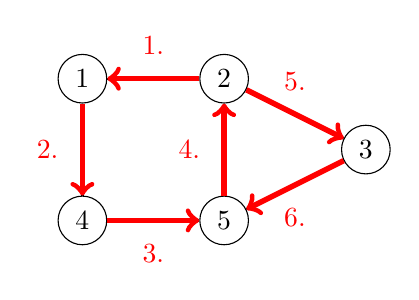
\begin{tikzpicture}[scale=0.9]
\node[draw, circle] (1) at (1,5) {$1$};
\node[draw, circle] (2) at (3,5) {$2$};
\node[draw, circle] (3) at (5,4) {$3$};
\node[draw, circle] (4) at (1,3) {$4$};
\node[draw, circle] (5) at (3,3) {$5$};

\path[draw,thick,-] (1) -- (2);
\path[draw,thick,-] (2) -- (3);
\path[draw,thick,-] (1) -- (4);
\path[draw,thick,-] (3) -- (5);
\path[draw,thick,-] (2) -- (5);
\path[draw,thick,-] (4) -- (5);

\path[draw=red,thick,->,line width=2pt] (2) -- node[font=\small,label={[red]north:1.}] {} (1);
\path[draw=red,thick,->,line width=2pt] (1) -- node[font=\small,label={[red]left:2.}] {} (4);
\path[draw=red,thick,->,line width=2pt] (4) -- node[font=\small,label={[red]south:3.}] {} (5);
\path[draw=red,thick,->,line width=2pt] (5) -- node[font=\small,label={[red]left:4.}] {} (2);
\path[draw=red,thick,->,line width=2pt] (2) -- node[font=\small,label={[red]north:5.}] {} (3);
\path[draw=red,thick,->,line width=2pt] (3) -- node[font=\small,label={[red]south:6.}] {} (5);
\end{tikzpicture}
\end{center}

\index{Hamiltonin polku}
Vastaavasti Hamiltonin polku (\textit{Hamiltonian path})
on verkossa oleva polku,
joka kulkee tarkalleen kerran jokaisen solmun kautta.
Yllä olevassa verkossa on esimerkiksi
Hamiltonin polku solmusta 1 solmuun 3:
\begin{center}
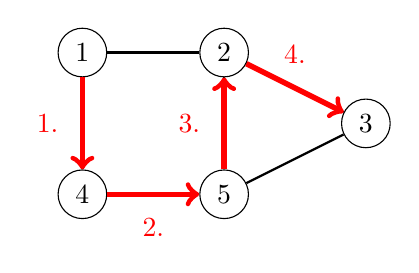
\begin{tikzpicture}[scale=0.9]
\node[draw, circle] (1) at (1,5) {$1$};
\node[draw, circle] (2) at (3,5) {$2$};
\node[draw, circle] (3) at (5,4) {$3$};
\node[draw, circle] (4) at (1,3) {$4$};
\node[draw, circle] (5) at (3,3) {$5$};

\path[draw,thick,-] (1) -- (2);
\path[draw,thick,-] (2) -- (3);
\path[draw,thick,-] (1) -- (4);
\path[draw,thick,-] (3) -- (5);
\path[draw,thick,-] (2) -- (5);
\path[draw,thick,-] (4) -- (5);

\path[draw=red,thick,->,line width=2pt] (1) -- node[font=\small,label={[red]left:1.}] {} (4);
\path[draw=red,thick,->,line width=2pt] (4) -- node[font=\small,label={[red]south:2.}] {} (5);
\path[draw=red,thick,->,line width=2pt] (5) -- node[font=\small,label={[red]left:3.}] {} (2);
\path[draw=red,thick,->,line width=2pt] (2) -- node[font=\small,label={[red]north:4.}] {} (3);
\end{tikzpicture}
\end{center}

\index{Eulerin kierros}
\index{Hamiltonin kierros}
Jos Eulerin polun alku- ja loppusolmu on sama,
kyseessä on Eulerin kierros (\textit{Eulerian circuit}).
Vastaavasti jos Hamiltonin polun alku- ja loppusolmu on sama,
kyseessä on Hamiltonin kierros (\textit{Hamiltonian circuit}).

Yllä olevassa verkossa ei ole Eulerin kierrosta,
mutta siinä on Hamiltonin kierros, jonka alku- ja loppusolmu on solmu 1:
\begin{center}
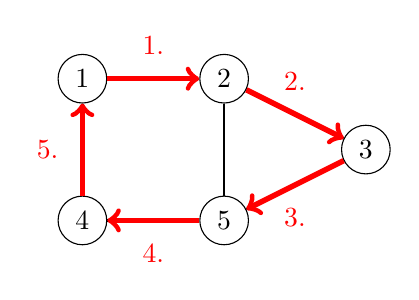
\begin{tikzpicture}[scale=0.9]
\node[draw, circle] (1) at (1,5) {$1$};
\node[draw, circle] (2) at (3,5) {$2$};
\node[draw, circle] (3) at (5,4) {$3$};
\node[draw, circle] (4) at (1,3) {$4$};
\node[draw, circle] (5) at (3,3) {$5$};

\path[draw,thick,-] (1) -- (2);
\path[draw,thick,-] (2) -- (3);
\path[draw,thick,-] (1) -- (4);
\path[draw,thick,-] (3) -- (5);
\path[draw,thick,-] (2) -- (5);
\path[draw,thick,-] (4) -- (5);

\path[draw=red,thick,->,line width=2pt] (1) -- node[font=\small,label={[red]north:1.}] {} (2);
\path[draw=red,thick,->,line width=2pt] (2) -- node[font=\small,label={[red]north:2.}] {} (3);
\path[draw=red,thick,->,line width=2pt] (3) -- node[font=\small,label={[red]south:3.}] {} (5);
\path[draw=red,thick,->,line width=2pt] (5) -- node[font=\small,label={[red]south:4.}] {} (4);
\path[draw=red,thick,->,line width=2pt] (4) -- node[font=\small,label={[red]left:5.}] {} (1);
\end{tikzpicture}
\end{center}

Vaikka Eulerin ja Hamiltonin polku ovat samantapaisia käsitteitä,
niihin liittyy laskennallisesti hyvin erilaisia ongelmia.
Näemme seuraavaksi, että yksinkertainen verkon rakenteeseen liittyvä
ehto ratkaisee, onko verkossa Eulerin polkua,
ja myönteisessä tapauksessa on helppoa etsiä jokin polku verkosta.

Hamiltonin polun tapauksessa tilanne on kuitenkin täysin toinen:
ei tunneta mitään tehokasta menetelmää, jolla voi selvittää,
onko verkossa Hamiltonin polkua, vaan kyseessä on NP-täydellinen ongelma.
Ainoat tunnetut yleiset menetelmät Hamiltonin polun muodostamiseen perustuvat
raakaan voimaan.

\section{Eulerin polku}

Osoittautuu, että Eulerin polun ja kierroksen olemassaolo riippuu verkon solmujen asteista.
Solmun aste on sen naapurien määrä eli niiden solmujen määrä,
jotka ovat yhteydessä solmuun kaarella.

Jos verkko on suuntaamaton,
siinä on Eulerin kierros tarkalleen silloin,
kun kaikki kaaret ovat samassa yhtenäisessä
komponentissa ja jokaisen solmun aste on parillinen.
Lisäksi jos tasan kahden solmun aste on pariton,
verkossa ei ole Eulerin kierrosta, mutta siinä
on Eulerin polku, jonka päätesolmut ovat
paritonasteiset solmut.

\begin{samepage}
Esimerkiksi verkossa
\begin{center}
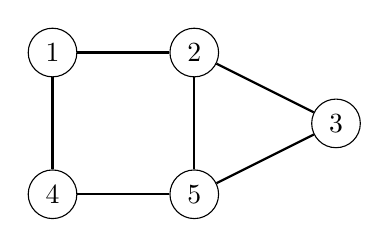
\begin{tikzpicture}[scale=0.9]
\node[draw, circle] (1) at (1,5) {$1$};
\node[draw, circle] (2) at (3,5) {$2$};
\node[draw, circle] (3) at (5,4) {$3$};
\node[draw, circle] (4) at (1,3) {$4$};
\node[draw, circle] (5) at (3,3) {$5$};

\path[draw,thick,-] (1) -- (2);
\path[draw,thick,-] (2) -- (3);
\path[draw,thick,-] (1) -- (4);
\path[draw,thick,-] (3) -- (5);
\path[draw,thick,-] (2) -- (5);
\path[draw,thick,-] (4) -- (5);
\end{tikzpicture}
\end{center}
\end{samepage}

solmujen 1, 3 ja 4 aste on 2 ja solmujen 2 ja 5 aste on 3.
Tarkalleen kahden solmun aste on pariton,
joten verkossa on Eulerin polku solmujen 2 ja 5 välillä,
mutta verkossa ei ole Eulerin kierrosta.

Jos verkko on suunnattu, tilanne on hieman hankalampi.
Silloin Eulerin polun ja kierroksen olemassaoloon
vaikuttavat solmujen lähtö- ja tuloasteet.
Solmun lähtöaste on solmusta lähtevien kaarten määrä,
ja vastaavasti solmun tuloaste on solmuun tulevien kaarten määrä.

Suunnatussa verkossa on Eulerin kierros, jos
kaikki kaaret ovat samassa vahvasti yhtenäisessä
komponentissa ja joka solmun lähtöaste ja tuloaste on sama.
Lisäksi verkossa on Eulerin polku,
jos alkusolmussa lähtöaste on yhden suurempi kuin tuloaste,
loppusolmussa tuloaste on yhden suurempi kuin lähtöaste
ja muissa solmuissa lähtö- ja tuloasteet ovat samat.

Esimerkiksi verkossa
\begin{center}
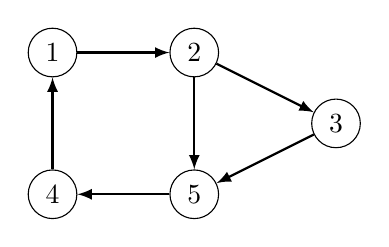
\begin{tikzpicture}[scale=0.9]
\node[draw, circle] (1) at (1,5) {$1$};
\node[draw, circle] (2) at (3,5) {$2$};
\node[draw, circle] (3) at (5,4) {$3$};
\node[draw, circle] (4) at (1,3) {$4$};
\node[draw, circle] (5) at (3,3) {$5$};

\path[draw,thick,->,>=latex] (1) -- (2);
\path[draw,thick,->,>=latex] (2) -- (3);
\path[draw,thick,->,>=latex] (4) -- (1);
\path[draw,thick,->,>=latex] (3) -- (5);
\path[draw,thick,->,>=latex] (2) -- (5);
\path[draw,thick,->,>=latex] (5) -- (4);
\end{tikzpicture}
\end{center}
solmuissa 1, 3 ja 4 sekä lähtöaste että tuloaste on 1.
Solmussa 2 tuloaste on 1 ja lähtöaste on 2,
kun taas solmussa 5 tulosate on 2 ja lähtöaste on 1.
Niinpä verkossa on Eulerin polku solmusta 2 solmuun 5:
\begin{center}
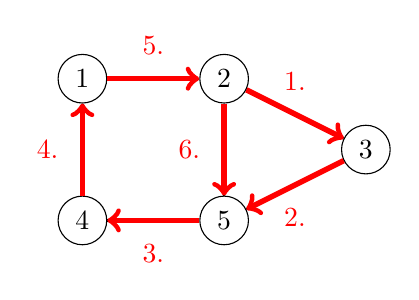
\begin{tikzpicture}[scale=0.9]
\node[draw, circle] (1) at (1,5) {$1$};
\node[draw, circle] (2) at (3,5) {$2$};
\node[draw, circle] (3) at (5,4) {$3$};
\node[draw, circle] (4) at (1,3) {$4$};
\node[draw, circle] (5) at (3,3) {$5$};

\path[draw,thick,-] (1) -- (2);
\path[draw,thick,-] (2) -- (3);
\path[draw,thick,-] (1) -- (4);
\path[draw,thick,-] (3) -- (5);
\path[draw,thick,-] (2) -- (5);
\path[draw,thick,-] (4) -- (5);

\path[draw=red,thick,->,line width=2pt] (2) -- node[font=\small,label={[red]north:1.}] {} (3);
\path[draw=red,thick,->,line width=2pt] (3) -- node[font=\small,label={[red]south:2.}] {} (5);
\path[draw=red,thick,->,line width=2pt] (5) -- node[font=\small,label={[red]south:3.}] {} (4);
\path[draw=red,thick,->,line width=2pt] (4) -- node[font=\small,label={[red]left:4.}] {} (1);
\path[draw=red,thick,->,line width=2pt] (1) -- node[font=\small,label={[red]north:5.}] {} (2);
\path[draw=red,thick,->,line width=2pt] (2) -- node[font=\small,label={[red]left:6.}] {} (5);
\end{tikzpicture}
\end{center}

\subsubsection{Algoritmi}

Seuraavaksi esitettävä algoritmi muodostaa Eulerin kierroksen
suuntaamattomassa verkossa.
Algoritmi olettaa, että kaikki kaaret ovat samassa
komponentissa ja jokaisen solmun aste on parillinen.

Jos verkossa on kaksi paritonasteista solmua,
samalla algoritmilla voi myös muodostaa
Eulerin polun lisäämällä kaaren
paritonasteisten solmujen välille.
Tämän jälkeen verkosta voi etsiä Eulerin kierroksen,
ja lopuksi Eulerin kierroksesta saa Eulerin polun
poistamalla ylimääräisen kaaren.

Algoritmi muodostaa ensin verkkoon jonkin kierroksen,
johon kuuluu osa verkon kaarista.
Sen jälkeen algoritmi alkaa laajentaa kierrosta
lisäämällä sen osaksi uusia alikierroksia.
Tämä jatkuu niin kauan, kunnes kaikki kaaret kuuluvat
kierrokseen ja siitä on tullut Eulerin kierros.

Algoritmi laajentaa kierrosta valitsemalla jonkin
kierrokseen kuuluvan solmun $x$,
jonka kaikki kaaret eivät ole vielä mukana kierroksessa.
Algoritmi muodostaa solmusta $x$ alkaen uuden polun
kulkien vain sellaisia kaaria, jotka eivät ole
mukana kierroksessa.
Koska jokaisen solmun aste on parillinen,
ennemmin tai myöhemmin polku palaa takaisin solmuun.

\begin{samepage}
Tarkastellaan algoritmin toimintaa seuraavassa verkossa:
\begin{center}
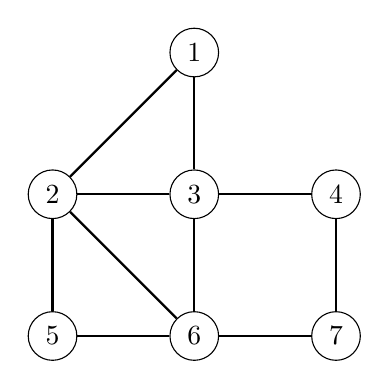
\begin{tikzpicture}[scale=0.9]
\node[draw, circle] (1) at (3,5) {$1$};
\node[draw, circle] (2) at (1,3) {$2$};
\node[draw, circle] (3) at (3,3) {$3$};
\node[draw, circle] (4) at (5,3) {$4$};
\node[draw, circle] (5) at (1,1) {$5$};
\node[draw, circle] (6) at (3,1) {$6$};
\node[draw, circle] (7) at (5,1) {$7$};

\path[draw,thick,-] (1) -- (2);
\path[draw,thick,-] (1) -- (3);
\path[draw,thick,-] (2) -- (3);
\path[draw,thick,-] (2) -- (5);
\path[draw,thick,-] (2) -- (6);
\path[draw,thick,-] (3) -- (4);
\path[draw,thick,-] (3) -- (6);
\path[draw,thick,-] (4) -- (7);
\path[draw,thick,-] (5) -- (6);
\path[draw,thick,-] (6) -- (7);
\end{tikzpicture}
\end{center}
\end{samepage}

\begin{samepage}
Oletetaan, että algoritmi aloittaa
ensimmäisen kierroksen solmusta 1.
Siitä syntyy kierros $1 \rightarrow 2 \rightarrow 3 \rightarrow 1$:
\begin{center}
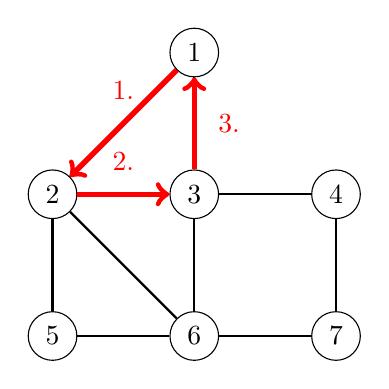
\begin{tikzpicture}[scale=0.9]
\node[draw, circle] (1) at (3,5) {$1$};
\node[draw, circle] (2) at (1,3) {$2$};
\node[draw, circle] (3) at (3,3) {$3$};
\node[draw, circle] (4) at (5,3) {$4$};
\node[draw, circle] (5) at (1,1) {$5$};
\node[draw, circle] (6) at (3,1) {$6$};
\node[draw, circle] (7) at (5,1) {$7$};

\path[draw,thick,-] (1) -- (2);
\path[draw,thick,-] (1) -- (3);
\path[draw,thick,-] (2) -- (3);
\path[draw,thick,-] (2) -- (5);
\path[draw,thick,-] (2) -- (6);
\path[draw,thick,-] (3) -- (4);
\path[draw,thick,-] (3) -- (6);
\path[draw,thick,-] (4) -- (7);
\path[draw,thick,-] (5) -- (6);
\path[draw,thick,-] (6) -- (7);

\path[draw=red,thick,->,line width=2pt] (1) -- node[font=\small,label={[red]north:1.}] {} (2);
\path[draw=red,thick,->,line width=2pt] (2) -- node[font=\small,label={[red]north:2.}] {} (3);
\path[draw=red,thick,->,line width=2pt] (3) -- node[font=\small,label={[red]east:3.}] {} (1);
\end{tikzpicture}
\end{center}
\end{samepage}

Seuraavaksi algoritmi lisää mukaan kierroksen
$2 \rightarrow 5 \rightarrow 6 \rightarrow 2$:
\begin{center}
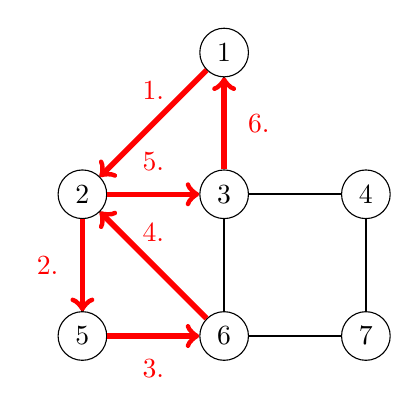
\begin{tikzpicture}[scale=0.9]
\node[draw, circle] (1) at (3,5) {$1$};
\node[draw, circle] (2) at (1,3) {$2$};
\node[draw, circle] (3) at (3,3) {$3$};
\node[draw, circle] (4) at (5,3) {$4$};
\node[draw, circle] (5) at (1,1) {$5$};
\node[draw, circle] (6) at (3,1) {$6$};
\node[draw, circle] (7) at (5,1) {$7$};

\path[draw,thick,-] (1) -- (2);
\path[draw,thick,-] (1) -- (3);
\path[draw,thick,-] (2) -- (3);
\path[draw,thick,-] (2) -- (5);
\path[draw,thick,-] (2) -- (6);
\path[draw,thick,-] (3) -- (4);
\path[draw,thick,-] (3) -- (6);
\path[draw,thick,-] (4) -- (7);
\path[draw,thick,-] (5) -- (6);
\path[draw,thick,-] (6) -- (7);

\path[draw=red,thick,->,line width=2pt] (1) -- node[font=\small,label={[red]north:1.}] {} (2);
\path[draw=red,thick,->,line width=2pt] (2) -- node[font=\small,label={[red]west:2.}] {} (5);
\path[draw=red,thick,->,line width=2pt] (5) -- node[font=\small,label={[red]south:3.}] {} (6);
\path[draw=red,thick,->,line width=2pt] (6) -- node[font=\small,label={[red]north:4.}] {} (2);
\path[draw=red,thick,->,line width=2pt] (2) -- node[font=\small,label={[red]north:5.}] {} (3);
\path[draw=red,thick,->,line width=2pt] (3) -- node[font=\small,label={[red]east:6.}] {} (1);
\end{tikzpicture}
\end{center}

Lopuksi algoritmi lisää mukaan kierroksen
$6 \rightarrow 3 \rightarrow 4 \rightarrow 7 \rightarrow 6$:
\begin{center}
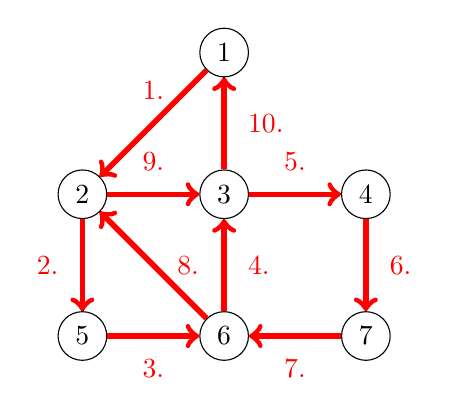
\begin{tikzpicture}[scale=0.9]
\node[draw, circle] (1) at (3,5) {$1$};
\node[draw, circle] (2) at (1,3) {$2$};
\node[draw, circle] (3) at (3,3) {$3$};
\node[draw, circle] (4) at (5,3) {$4$};
\node[draw, circle] (5) at (1,1) {$5$};
\node[draw, circle] (6) at (3,1) {$6$};
\node[draw, circle] (7) at (5,1) {$7$};

\path[draw,thick,-] (1) -- (2);
\path[draw,thick,-] (1) -- (3);
\path[draw,thick,-] (2) -- (3);
\path[draw,thick,-] (2) -- (5);
\path[draw,thick,-] (2) -- (6);
\path[draw,thick,-] (3) -- (4);
\path[draw,thick,-] (3) -- (6);
\path[draw,thick,-] (4) -- (7);
\path[draw,thick,-] (5) -- (6);
\path[draw,thick,-] (6) -- (7);

\path[draw=red,thick,->,line width=2pt] (1) -- node[font=\small,label={[red]north:1.}] {} (2);
\path[draw=red,thick,->,line width=2pt] (2) -- node[font=\small,label={[red]west:2.}] {} (5);
\path[draw=red,thick,->,line width=2pt] (5) -- node[font=\small,label={[red]south:3.}] {} (6);
\path[draw=red,thick,->,line width=2pt] (6) -- node[font=\small,label={[red]east:4.}] {} (3);
\path[draw=red,thick,->,line width=2pt] (3) -- node[font=\small,label={[red]north:5.}] {} (4);
\path[draw=red,thick,->,line width=2pt] (4) -- node[font=\small,label={[red]east:6.}] {} (7);
\path[draw=red,thick,->,line width=2pt] (7) -- node[font=\small,label={[red]south:7.}] {} (6);
\path[draw=red,thick,->,line width=2pt] (6) -- node[font=\small,label={[red]right:8.}] {} (2);
\path[draw=red,thick,->,line width=2pt] (2) -- node[font=\small,label={[red]north:9.}] {} (3);
\path[draw=red,thick,->,line width=2pt] (3) -- node[font=\small,label={[red]east:10.}] {} (1);
\end{tikzpicture}
\end{center}

Nyt kaikki kaaret ovat kierroksessa,
joten Eulerin kierros on valmis.

\subsubsection{Toteutus}

Edellä kuvattu algoritmi on mukavaa toteuttaa
niin, että solmujen vieruslistat on tallennettu joukkoina

\begin{lstlisting}
set<int> v[N];
\end{lstlisting}

jolloin verkosta on helppoa poistaa kahden solmun
välinen kaari, kun se tulee mukaan kierrokseen.

Seuraava koodi muodostaa Eulerin kierroksen
solmusta $x$ alkaen.
Se käyttää apuna pinoa \texttt{s},
jossa on aluksi vain kierroksen alkusolmu.
Jos pinon ylimmän solmun $u$ aste on 0,
se lisätään Eulerin kierrokseen.
Muuten pinon päälle lisätään uusi alikierros
solmusta $u$ alkaen ja kaikki alikierrokseen
kuuluvat kaaret poistetaan verkosta.

\begin{lstlisting}
stack<int> s;
s.push(x);
while (!s.empty()) {
    int u = s.top(); s.pop();
    if (v[u].size() == 0) {
        // lisää solmu u Eulerin kierrokseen
    } else {
        int a = u;
        s.push(a);
        do {
            int b = *v[a].begin();
            v[a].erase(b);
            v[b].erase(a);
            s.push(b);
            a = b;
        } while (a != u);
    }
}
\end{lstlisting}
Toteutuksen aikavaativuus on $O(n+m \log n)$,
koska se käy läpi kaikki solmut ja kaaret
ja kunkin kaaren poistaminen vie aikaa $O(\log n)$.
Myös toteutus ajassa $O(n+m)$
on mahdollista mutta vaikeampaa.
Tämä vaatii verkon esittämistä niin,
että kaaria pystyy poistamaan ajassa $O(1)$.

\section{De Bruijnin jono}

\index{de Bruijnin jono}

\begin{task}
Annettuna on merkistö,
jossa on $k$ merkkiä, sekä pituus $n$.
Mikä on lyhin merkkijono, jossa on osana
kaikki $n$ merkin yhdistelmät?
\end{task}

Esimerkiksi jos merkistö on $\{0,1\}$
ja $n=3$, lyhin merkkijono on 10-merkkinen
ja yksi tapa muodostaa se on 0001011100.
Merkkijonon osana ovat kaikki 3 merkin yhdistelmät
000, 001, 010, 011, 100, 101, 110 ja 111.

Osoittautuu, että lyhimmän merkkijonon
pituus on aina $k^n+n-1$ ja merkkijono
vastaa Eulerin kierrosta sopivasti
muodostetussa verkossa.
Tällaista merkkijonoa kutsutaan
de Bruijnin jonoksi (\textit{de Bruijn sequence}).

Ideana on muodostaa verkko niin,
että jokaisessa solmussa on $n-1$
merkin yhdistelmä ja liikkuminen
kaarta pitkin muodostaa uuden
$n$ merkin yhdistelmän.
Esimerkin tapauksessa verkosta tulee seuraava:
\\
\begin{center}
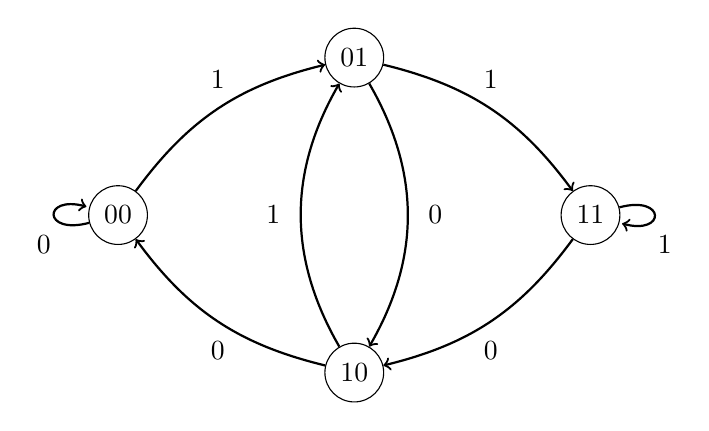
\begin{tikzpicture}
\node[draw, circle] (00) at (-3,0) {00};
\node[draw, circle] (11) at (3,0) {11};
\node[draw, circle] (01) at (0,2) {01};
\node[draw, circle] (10) at (0,-2) {10};

\path[draw,thick,->] (00) edge [bend left=20] node[font=\small,label=1] {} (01);
\path[draw,thick,->] (01) edge [bend left=20] node[font=\small,label=1] {} (11);
\path[draw,thick,->] (11) edge [bend left=20] node[font=\small,label=below:0] {} (10);
\path[draw,thick,->] (10) edge [bend left=20] node[font=\small,label=below:0] {} (00);

\path[draw,thick,->] (01) edge [bend left=30] node[font=\small,label=right:0] {} (10);
\path[draw,thick,->] (10) edge [bend left=30] node[font=\small,label=left:1] {} (01);

\path[draw,thick,-] (00) edge [loop left] node[font=\small,label=below:0] {} (00);
\path[draw,thick,-] (11) edge [loop right] node[font=\small,label=below:1] {} (11);
\end{tikzpicture}
\end{center}

Eulerin kierros tässä verkossa tuottaa merkkijonon,
joka sisältää kaikki $n$ merkin yhdistelmät,
kun mukaan otetaan aloitussolmun merkit sekä
kussakin kaaressa olevat merkit.
Aloitussolmussa on $n-1$ merkkiä ja kaarissa
on $k^n$ merkkiä, joten tuloksena on
lyhin mahdollinen merkkijono.
